\chapter{Pin Control Defense}
\label{chap:defense}

This chapter proposes a possible countermeasure to Pin Control Attack.
First, it describes the overall design of Pin Control Defense, showing different approaches to tackle the attack at different levels
and explaining our design choices. Second, it contains a detailed report of the defense implementation.


\section{Design}
We report the design phase below, starting from a preliminary analysis of the problem to a discussion of different possible solutions.
Then, a detailed description of the defense architecture concludes the section.


\subsection{Preliminary analysis}
\label{sec:pre-analysis}

The main goal of our defense is to detect and hinder Pin Control Attack while being able to not consume the limited resources inside the target system,
and to not affect real-time operations. The timing of the operations is fundamental in systems like PLCs, on which the minimum delay may alter the physical process.

We make the same assumptions contained in the threat model of \mysec{sec:threat-model}.
Therefore, we assume that the system, and our defense as well, is protected by the previously discussed HIDSs.
Starting from the analysis reported in \mychap{chap:attack}, we identify the I/O configuration as the main resource we aim to protect from Pin Control Attack.
To target I/O configuration, the attacker may use other system capabilities, such as virtual address mapping and debug registers.
First of all, we define the following components of a SoC, to which we refer several times in the rest of the paper:
\begin{itemize}
	\item \itemname{I/O subsystem}: the subsystem that controls the I/O configuration. I/O configuration is defined as the set of all the control registers
		actively used by the SoC, whose unauthorised modification may have direct or indirect effects on the controlled process.
		In particular, we are interested into pin control registers, which directly determine the behaviour of the SoC I/O pins.
		However, a SoC typically contains many devices and controllers which may be in charge of a subset of I/O pins. In other words, some pins
		can be multiplexed to specific devices inside the SoC. Since these devices are programmed through their own control registers,
		altering these registers may indirectly affect I/O pins as well. Thus, both pin control registers and device control registers
		are considered as part of the I/O configuration. The attacker who has knowledge of the system and its I/O peripherals may access
		all these registers to alter the physical process.
	\item \itemname{Debug subsystem}: the SoC subsystem that enables debug capabilities for the operating system and its processes.
		Typically, it consists of a set of registers, called \emph{debug registers}, inside the processor of the SoC.
		The operating system may provide an interface to access them, both for kernel side and user side.
		The attacker may leverage the debug subsystem to obtain accurate timing information and conduct more sophisticated attacks,
		either using the interface provided by the operating system or the low-level processor instructions directly (depending on its privilege level).
	\item \itemname{Mapping subsystem}: the system that manages mappings between physical and virtual addresses, both for kernel and user space.
		It is typically supported by the Memory Management Unit (MMU) in hardware, and by the operating system in software. Within the context of a PLC,
		the runtime may use this subsystem to configure the I/O and to perform read/write operations. An attacker can access physical I/O addresses
		(thus, I/O configuration) either by requesting a new mapping to the system or by using an already existing mapping.
\end{itemize}

Given the architecture described in \mysec{sec:embed-arch}, protecting I/O configuration is not straightforward because the hardware lacks
any protection mechanism related to the I/O subsystem. For instance, the SoC might generate a trap for each modification to I/O registers.
However, this approach would not be reasonable, because of the huge overhead imposed to any I/O access.
Alternatively, a trap could be generated only when an I/O access is malicious. For example, to prevent pin configuration attack,
a trap signal might be delivered to the CPU when the internal signal of a pin is different from the external one, meaning that the pin is misconfigured.
A similar approach may be used for pin multiplexing, by checking the internal signal connected to the multiplexed device.
Unfortunately, since these approaches would require significant hardware modifications, with subsequent updates of all the SoC drivers, they are very unlikely to be applied.

Thus, we need to define an alternative approach that does not have the above limitations: it must be easily applicable and have a minimal overhead.
Since the hardware-based solution is unpractical, we analysed the possible software-based solutions.
In order to choose the best strategy against Pin Control Attack, we compared the following approaches, as proposed in \cite{ghostplc}:
\begin{enumerate}
	\item monitoring I/O configuration to detect changes;
	\item monitoring the use of debug registers;
	\item monitoring the mapping requests targeting I/O configuration;
	\item monitoring performance overhead;
	\item using a trusted execution environment.
\end{enumerate}
These approaches are not mutually exclusive, and may be used simultaneously to get a higher protection level.
In this work, we decided to design and implement the first three approaches in combination, because they directly protect the three different resources that the attacker may use.
Thus, they represent a good minimum set of countermeasures capable of raising the bar for the attacker (see \mysec{sec:def-arch}).
Our solution, however, may be extended to include the last two approaches as well, to cover some existing limitations (see \mysec{sec:def-sec}).
Before describing our design phase, we briefly discuss these two further protections in the following sections.


\subsubsection{Monitoring performance overhead}

A detection system based on performance monitoring may be useful to add a further protection, especially against the attack variant
which uses debug registers. In general, such a monitor would be also useful for other kind of attacks targeting PLCs, because these systems cyclically performs
a limited amount of well-known operations. This simplifies the detection of any deviation from the standard behaviour.
In our case, a performance monitor would be helpful to cover those attacks that the first three strategies are not able to detect,
although, as discussed in the following sections, those are very limited cases.
Deploying a performance monitoring system, anyway, does not require very high effort because it can leverage \emph{Hardware Performance Counters} (HPC),
nowadays available in almost all the SoC processors. The most challenging part would be, of course, integrating the monitor with the PLC runtime.
When a new logic is uploaded to the PLC, a burst of operations are executed by the runtime to check the new logic code, apply the new configuration and start the logic.
These extra operations, of course, must not be labeled as malicious. Furthermore, once a new logic started, it may perform operations that are different
with respect to the previous one; therefore, the monitor should be able to recognise this change and update its statistics as well.


\subsubsection{Trusted execution environment}

A Trusted Execution Environment (TEE) is a particular set of hardware and software components providing security features,
such as isolated execution, integrity of Trusted Applications (TAs), and integrity and confidentiality of TAs assets \cite{tee}.
The TEE technology is based on the concept of partitioning a computing system into Secure and non-Secure world, where
the code running into non-Secure world cannot access the Secure partition.
A lot of effort has been put into the standardisation of the TEE, and some commercial solutions already exist,
such as Intel Trusted Execution Technology (TXT) \cite{intel-txt} and ARM TrustZone \cite{trustzone}.
Since embedded systems are our main target, we provide a brief description focused on the ARM TrustZone implementation.
In this technology, the physical memory is partitioned into Secure and non-Secure regions, and the processor core is divided into Secure and Non-secure virtual cores.
The virtual core is distinguished by the NSTID (Non-Secure Table IDentifier) bit associated with the current instruction,
while each instruction or data address (\ie each bus transaction) is marked with an NS bit.
The protection of the Secure world is guaranteed by checking all the accesses to memory or peripherals.
The Non-secure core can only access Non-secure memory regions, while the Secure world can use both Secure and Non-secure addresses.
This partitioning is parallel and independent from Supervisor/User modes available on the CPU. Therefore, each world has its own supervisor and user mode as well.
To improve the performance of this architecture, TLBs and caches may support the NS attribute for each entry as well.
This enables Secure and Non-secure entries to co-exist avoiding TLB and cache flushes on every switch between the two worlds.
The switching between Secure and Non-secure world is managed through a specific Secure Monitor Call (SMC) instruction,
which changes the core mode into Monitor Mode. The code executed into monitor mode is always Secure, and it basically performs the context switch
between the two virtual cores. If a Secure process is loaded, NSTID bit is set accordingly.
Since the Secure world may contain a whole parallel micro-kernel with trusted user applications, it may be possible
to deploy Pin Control Defense inside the trusted domain, protecting the defense itself from defense-aware attackers.
However, the overhead imposed by a trusted execution environment may be unacceptable for embedded systems with real-time constraints like PLCs.
Hence, the impact of this solution still needs to be investigated.


\subsection{Defense Architecture}
\label{sec:def-arch}

Based on the previous considerations, we designed a detection system which is able to protect against Pin Control Attack at three different levels,
corresponding to the SoC I/O, debug and map subsystems. The system is designed to run as part of the operating system, thus having kernel privilege level.
Its overall architecture is shown in \myfig{fig:defense}.
\begin{figure}[h]
\centerline{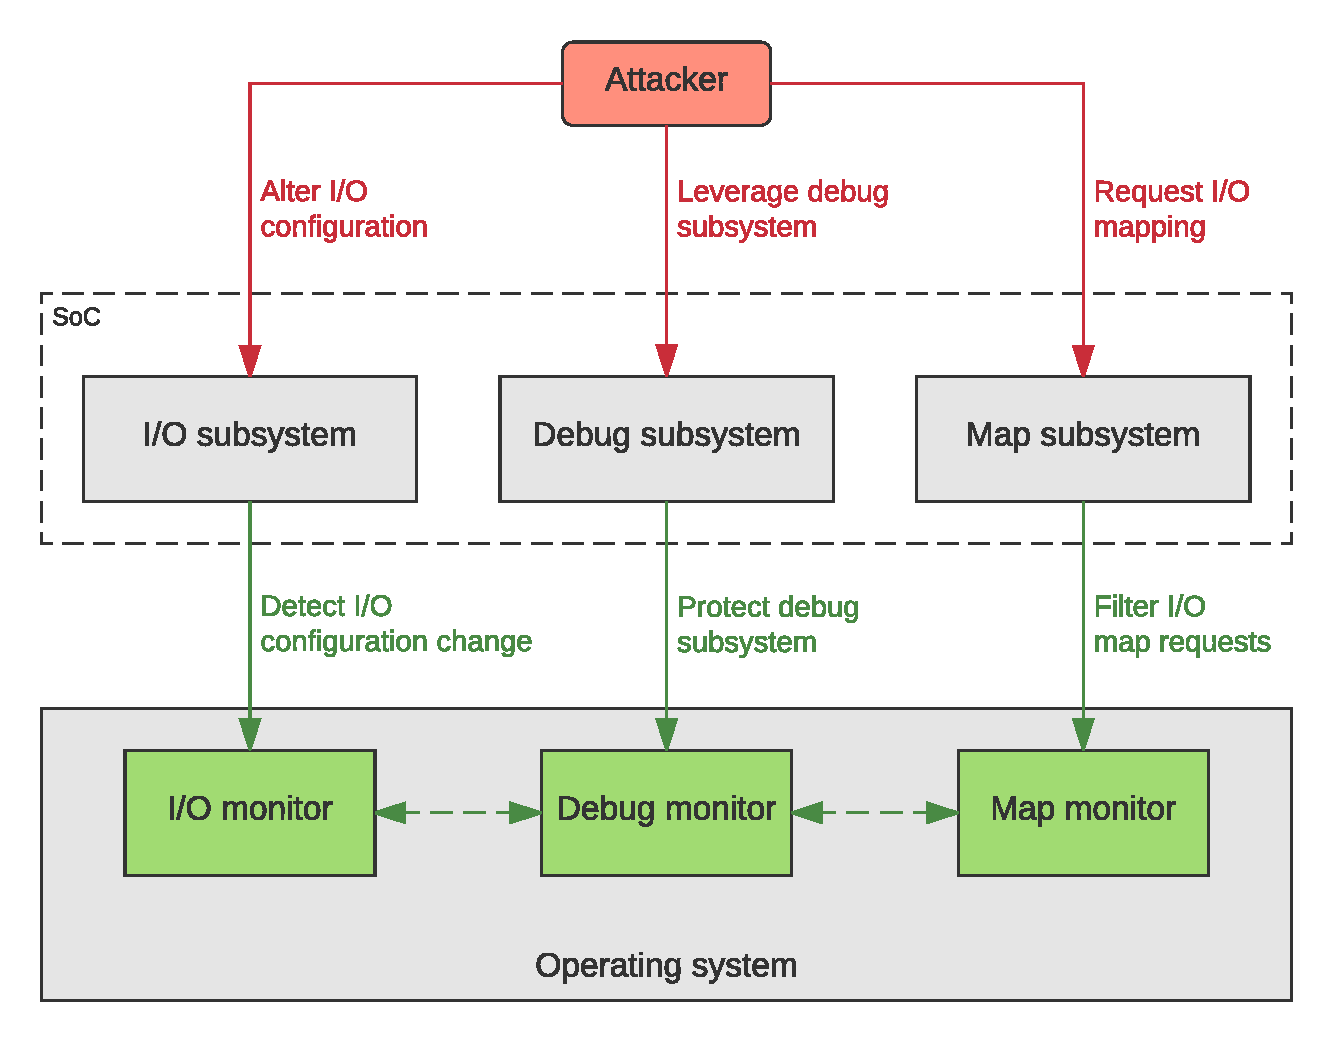
\includegraphics[width=0.8\textwidth]{res/defense}}
\caption{Pin Control Defense general architecture \label{fig:defense}}
\end{figure}
Considering that the attacker can possibly follow any of the paths highlighted in red in the figure,
our monitoring system has been divided into three main components:
\begin{itemize}
	\item \itemname{I/O monitor}: its purpose is to watch the I/O configuration, detect and react to any malicious change.
	\item \itemname{Debug monitor}: it aims to protect the debug subsystem from malicious usage.
	\item \itemname{Map monitor}: it acts as a filter for mapping requests targeting I/O memory.
\end{itemize}

Each monitor is responsible for reporting detection information related to any interesting event of the respective subsystem,
and reacting to these events according to its own configuration. The events are not necessarily due to Pin Control Attack,
\eg an I/O configuration change event may be caused by the PLC runtime.
Therefore, the I/O monitor should decide whether a particular I/O modification can be considered legitimate or not.
Debug and map monitors, instead, serve at least the following purposes:
\begin{itemize}
	\item \itemname{early detection}: the attack can be detected before it modifies the I/O configuration;
	\item \itemname{raising the bar}: they limit the attacker possibilities, by restricting the access to the corresponding subsystem;
	\item \itemname{reporting info}: they provide additional information, useful to figure out how an eventual attack has been conducted.
\end{itemize}
Since these modules are designed to be customisable, the actual effects depends on their configuration.
The following sections describe in more detail the design and the role of each module.


\subsection{I/O monitor}
\label{sec:io-design}

The I/O monitor plays the most critical role into our detection system.
Its main task is to cyclically check the values contained into I/O configuration registers, to verify that they are conforming with the logic currently loaded into the PLC.
If a change into a target register has been detected, it determines whether this modification is legal or not, according to a given trusted behaviour.
As discussed in \mysec{sec:plc-arch}, a new I/O configuration may come with a new PLC logic, and the PLC runtime must be able to apply the change without
having our defense to interfere.
Therefore, an automated mechanism able to distinguish between trusted and malicious configurations is needed.
This is not an easy problem, because an optimal solution would require an authentication between PLC runtime and I/O subsystem,
and this is not reasonable in our highly constrained system.

To tackle this problem, we designed the following strategy, which we used to implement the I/O monitor:
\begin{enumerate}
	\item define I/O configuration registers;
	\item define a trusted behavioural model of the I/O configuration;
	\item \label{enum:io-monitor} constantly monitor the I/O configuration to detect possible modifications;
	\item if a change is detected, verify whether it is conforming to the defined behaviour or not;
	\item if it is, accept the new configuration and go back to \ref{enum:io-monitor};
	\item otherwise, it is probably Pin Control Attack: react according to the configured monitor action and go back to \ref{enum:io-monitor}.
\end{enumerate}
The first step is to choose which registers should be included into the I/O configuration, \ie which registers should be protected.
This set of registers includes, ideally, all the registers whose modification may produce an effect on the physical process.
However, it is not always possible to define a behavioural model or enable the protection for each register. For instance,
some registers may be write-only (\eg pull-up/down registers), and there is no way to verify their current value.
Whether to include or not a register into I/O configuration should be decided case by case,
according to the protection feasibility and the possible effects of a malicious modification.

To define the behavioural model, it is required to determine the set of configuration registers actively used into the target system,
\ie the set of registers that may affect the physical process. Then, for each register (or for each bit of each register if necessary),
the model should define under which conditions the corresponding value may change. These conditions are highly dependent on the target implementation.
Generally speaking, they can be represented by simple time constraints (\eg the value cannot change twice within $\SI{20}{ms}$),
logical conditions (\eg the value must be conforming to the running PLC logic), a statistical model, or a combination of these.
Each condition can either provide an exact distinction between a trustworthy and a malicious modification (typically logical conditions),
or a heuristic only. For this purpose, we analyse in more detail the proposed logical condition, since it is able to completely exclude false positives.
The condition states that a change can be accepted only if the new I/O configuration is in line with the operations performed by the running PLC logic.
Checking this condition is feasible as long as enough knowledge of the PLC runtime is available. To obtain this knowledge, two ways are doable:
\begin{itemize}
	\item \itemname{reverse engineering}: by analysing the PLC software it is possible to dynamically obtain the required information from the running logic;
	\item \itemname{PLC runtime vendor collaboration}: if the PLC software is designed to be aware of the defense mechanism,
		it could better expose the required information to the I/O monitor at run-time, thus removing the need for reverse engineering.
\end{itemize}
Once the I/O monitor is able to determine which operations the PLC logic is carrying on, it can easily decide if an I/O configuration is malicious or not,
and can effectively detect Pin Control Attack (see our approach in \mysec{sec:io-impl}).
Note that, if the information on the current I/O operations is made available by the PLC runtime, the attacker can modify it as well while conducting the attack.
In this case, however, the attacker needs to modify the PLC logic, and this may be easily noticed if further protection mechanisms are provided by the PLC runtime.
Therefore, the attack would lose one of the features that made it stealth.

An important parameter to discuss is the time interval of the main monitor loop. Since no other mechanisms are provided by the hardware,
such as interrupts, we can only detect I/O configuration changes by cyclically checking its current values. Greater scanning intervals may give the attacker
enough time-window to reach its purpose. For instance, given a PLC scan cycle of $\SI{10}{ms}$ and a monitor interval of $\SI{50}{ms}$,
if the attack is able to synchronise itself with the monitor loop, it has enough time to alter $\left \lfloor{\frac{\SI{50}{ms}}{\SI{10}{ms}}}\right \rfloor = 5$
consecutive I/O operations and then restore the configuration back before getting noticed. Smaller intervals, instead, may cause too much performance overhead.
We provide our experimental results in \mychap{chap:results}.

Another challenging aspect of this approach is to decide which action the monitor should follow if an attack has been detected.
We distinguished at least three main reactions for I/O monitor:
\begin{itemize}
	\item report the event to the system;
	\item revert the configuration back to the last known before the attack;
	\item stop the control process.
\end{itemize}
The choice among these actions (or a combination of them) again depends on the target implementation.
Typically, reporting the event is the minimum that the monitor can do, while other reactions should be decided according to risk associated with the physical process
and to the monitor reliability. If a detection is proven to be correct, due to an exact condition,
then reverting the configuration back could be the best choice. Otherwise, if the detection condition is a heuristic and the risk is critical,
stopping the control process may be considered as a more cautious alternative.
In general, if a monitor only reports about events we call it \emph{passive}, otherwise it is an \emph{active} monitor.


\subsection{Debug monitor}
\label{sec:dr-design}

This monitor is responsible for protecting the debug subsystem from malicious usage. Debug registers may be used by the attacker to gain accurate timing
information about the PLC logic I/O operations.
Similarly to what the I/O monitor does, the debug monitor continuously watches the values contained into debug registers to detect malicious modifications.
In our design, we assumed that there is no need to use debug registers into the target PLC if it is already deployed into a real control system.
As confirmed by our experiments, they are actually never used.
Typically, the SoC debug subsystem may only be needed by PLC vendors during design and implementation of their own product.
Since the operating system may provide user level access to debug registers (\eg \verb|ptrace| API on Linux), we can simply disable this user interface.
However, there is no mechanism to permanently disable debug registers also at kernel-wide level.
To understand this problem, we need to distinguish the following two cases: the debug support can be either enabled or disabled into the kernel itself.
If it is enabled, the attacker may simply leverage the system interface to use debug registers from kernel space.
If debug support is disabled, an attacker who gains kernel level access (as in kernel module version of Pin Control Attack) can always re-enable them at run-time
by inserting its own debug exception handler into the OS interrupt vector table (see \cite{arm-evt,x86-idt}).
However, this kind of attack is already covered by the defenses assumed in our threat model, because it is a data hooking technique.
Thus, we designed the following monitor strategy, that is required only if debug support is enabled into the operating system:
\begin{enumerate}
	\item disable debug registers user space interface;
	\item \label{enum:debug-monitor} constantly monitor debug registers to detect possible modifications (from kernel space);
	\item if a change is detected, it is Pin Control Attack: react according to the configured monitor action and go back to \ref{enum:debug-monitor}.
\end{enumerate}
The strategy is (in part) a simplification of the I/O monitor approach, on which the trusted behavioural model assumes that debug registers never change in a production system.
Based on this assumption, the debug module allows our defense to provide an early detection of the attack, before I/O configuration is actually altered.
The discussion about the monitor time interval is the same as for the previous I/O monitor: a trade-off between attacker time-window and monitor overhead.

When an attack has been detected, restoring the previous values of debug registers is surely the best action to take,
because the assumption ensures that only malicious changes may occur.
Halting the PLC process, instead, is certainly not needed because the control process is not directly affected by a modification of the debug subsystem.
In any case, the event is reported to the system. To uniform the design, the debug monitor can be configured either as passive or active,
although the passive mode is strongly discouraged for the above reasons. If the monitor is active, it actually raises the bar for the attacker,
who cannot leverage debug registers anymore.


\subsection{Mapping monitor}
\label{sec:map-design}

As discussed in \mysec{sec:pre-analysis}, the attacker may either request a new mapping between physical and virtual memory, or re-use an existing one before
modifying I/O configuration. The map monitor leverages this fact, providing a further detection mechanism usable in combination with the previous two.
Typically, the operating system provides an interface, for user space, through which each process can map a physical address region to a corresponding virtual region.
In the following part of this document we refer to it as ``mapping interface''.
The actual mapping is performed inside the kernel, and the process receives a valid virtual address as result.
The attacker can leverage this mechanism to gain access to the I/O configuration registers from user space.
According to the implementation, the PLC runtime may use this mechanism as well, and if it does, the attacker may try to re-use the PLC runtime virtual address.
We distinguish at least two techniques to re-use existing virtual addresses:
\begin{itemize}
	\item exploit a remote code execution vulnerability on the PLC runtime owning the addresses;
	\item set debug register on PLC runtime virtual address (the debug handler will have access to the process virtual addresses).
\end{itemize}
We exclude the second technique, because it is already detectable by the debug monitor. The first one, instead, can only be counteracted by detecting the control flow attack itself.
Thus, the aim of this monitor is not to detect addresses re-using, which is out of our scope, but to monitor \emph{new} mapping requests.
To achieve the goal, we dynamically replace the functions belonging to the mapping interface with our own versions (hook).
We can summarise the strategy of the map monitor as follows:
\begin{enumerate}
	\item \label{enum:map-model} define a trusted behavioural model for I/O mapping requests of the PLC runtime;
	\item hook all the functions belonging to the mapping interface;
	\item at each new mapping request, verify whether the requested physical address range overlaps the I/O configuration region or not;
	\item if there is no overlap, forward the request to the original system function;
	\item if an overlapping region is detected, verify whether the request is conforming to the trusted behaviour or not;
	\item if it is, forward the request to the original system function;
	\item if it is not, it is probably Pin Control Attack: react according to the configured monitor action.
\end{enumerate}
The behavioural model of step \ref{enum:map-model} should describe if and how the mapping interface is used by the PLC runtime.
We analysed the behaviour of our target systems, with the following results:
\begin{itemize}
	\item Raspberry Pi: the CODESYS runtime un-maps and re-maps the I/O every time a new PLC logic is uploaded;
	\item Wago PLC: e!RUNTIME never maps physical I/O from user space, because it is managed by the system driver.
\end{itemize}
The next step of the strategy, function hooking, must satisfy at least the following requirements (see implementation in \mysec{sec:def-impl} for more details):
\begin{itemize}
	\item it must be efficient: mapping functions may be called many times by processes (\eg in Linux, they are used not only to map physical memory,
		but any file, device, etc.);
	\item considering the threat model discussed in \mysec{sec:threat-model}, it must be applied before the Autoscopy Jr. detection system is deployed;
		otherwise, our modification will be considered as malicious.
\end{itemize}

Finally, the reaction of the map monitor to an eventual detection depends on the PLC runtime behaviour. If the PLC runtime maps the I/O (as in Raspberry Pi),
then a mechanism to distinguish between good and malicious requests is needed. To accomplish this, we may list the following alternatives:
\begin{itemize}
	\item heuristic approach based on statistical data;
	\item integration of the defense with the PLC runtime.
\end{itemize}
Since the first approach cannot give an exact detection, the monitor may simply report the detection to the system.
The second approach, instead, may be implemented in different ways. For instance, the map monitor could provide a separate mapping interface
reserved only for the PLC runtime process.
In any case, if the system allows to have an exact detection mechanism, the monitor may directly deny the malicious request, factually raising the bar for the attacker.


\section{Implementation}
\label{sec:def-impl}

We describe here our implementation of the above strategies, discussing the engineering problems encountered and the adopted solutions.
Since the authors of the attack presented their work as ``Ghost in the PLC'' \cite{ghostplc}, we called our defense prototype implementation \emph{Ghostbuster}.
Ghostbuster is a kernel module written in C language, targeting Embedded Linux running on ARM architecture.
It is designed to be highly configurable and as architecture-independent as possible, following the guideline of the Linux kernel itself.
A portion of the code, \ie the lowest level code, is still dependent from the specific architecture (\eg ARM), but is separated from the general implementation template.
This allows Ghostbuster to be easily extendable to other architectures and SoCs running Linux. At the same time, we focused on maintaining the lowest overhead possible,
which is always crucial for PLCs. We proceed with the description of the overall architecture, and then we go deep into each module of the architecture.
Finally, we describe the usage of our kernel module.


\subsection{Implementation architecture}

The implementation architecture is based on the general one described in \mysec{sec:def-arch}. Thus, we implemented I/O, debug and map monitors.
Each one of them has been divided into two main parts, following the template method pattern: the main strategy and the sub-actions implementation.
The aim of this separation is to minimise the effort needed to deploy our defense into different systems, thus improving its portability.
In particular, we considered the following variables: each target system may have its own System on Chip, firmware and PLC runtime.
During the design part, we defined high-level monitor strategies, which allowed us to provide an abstraction adaptable to any Linux-based system,
independently from these variables.
\begin{figure}[h]
\centerline{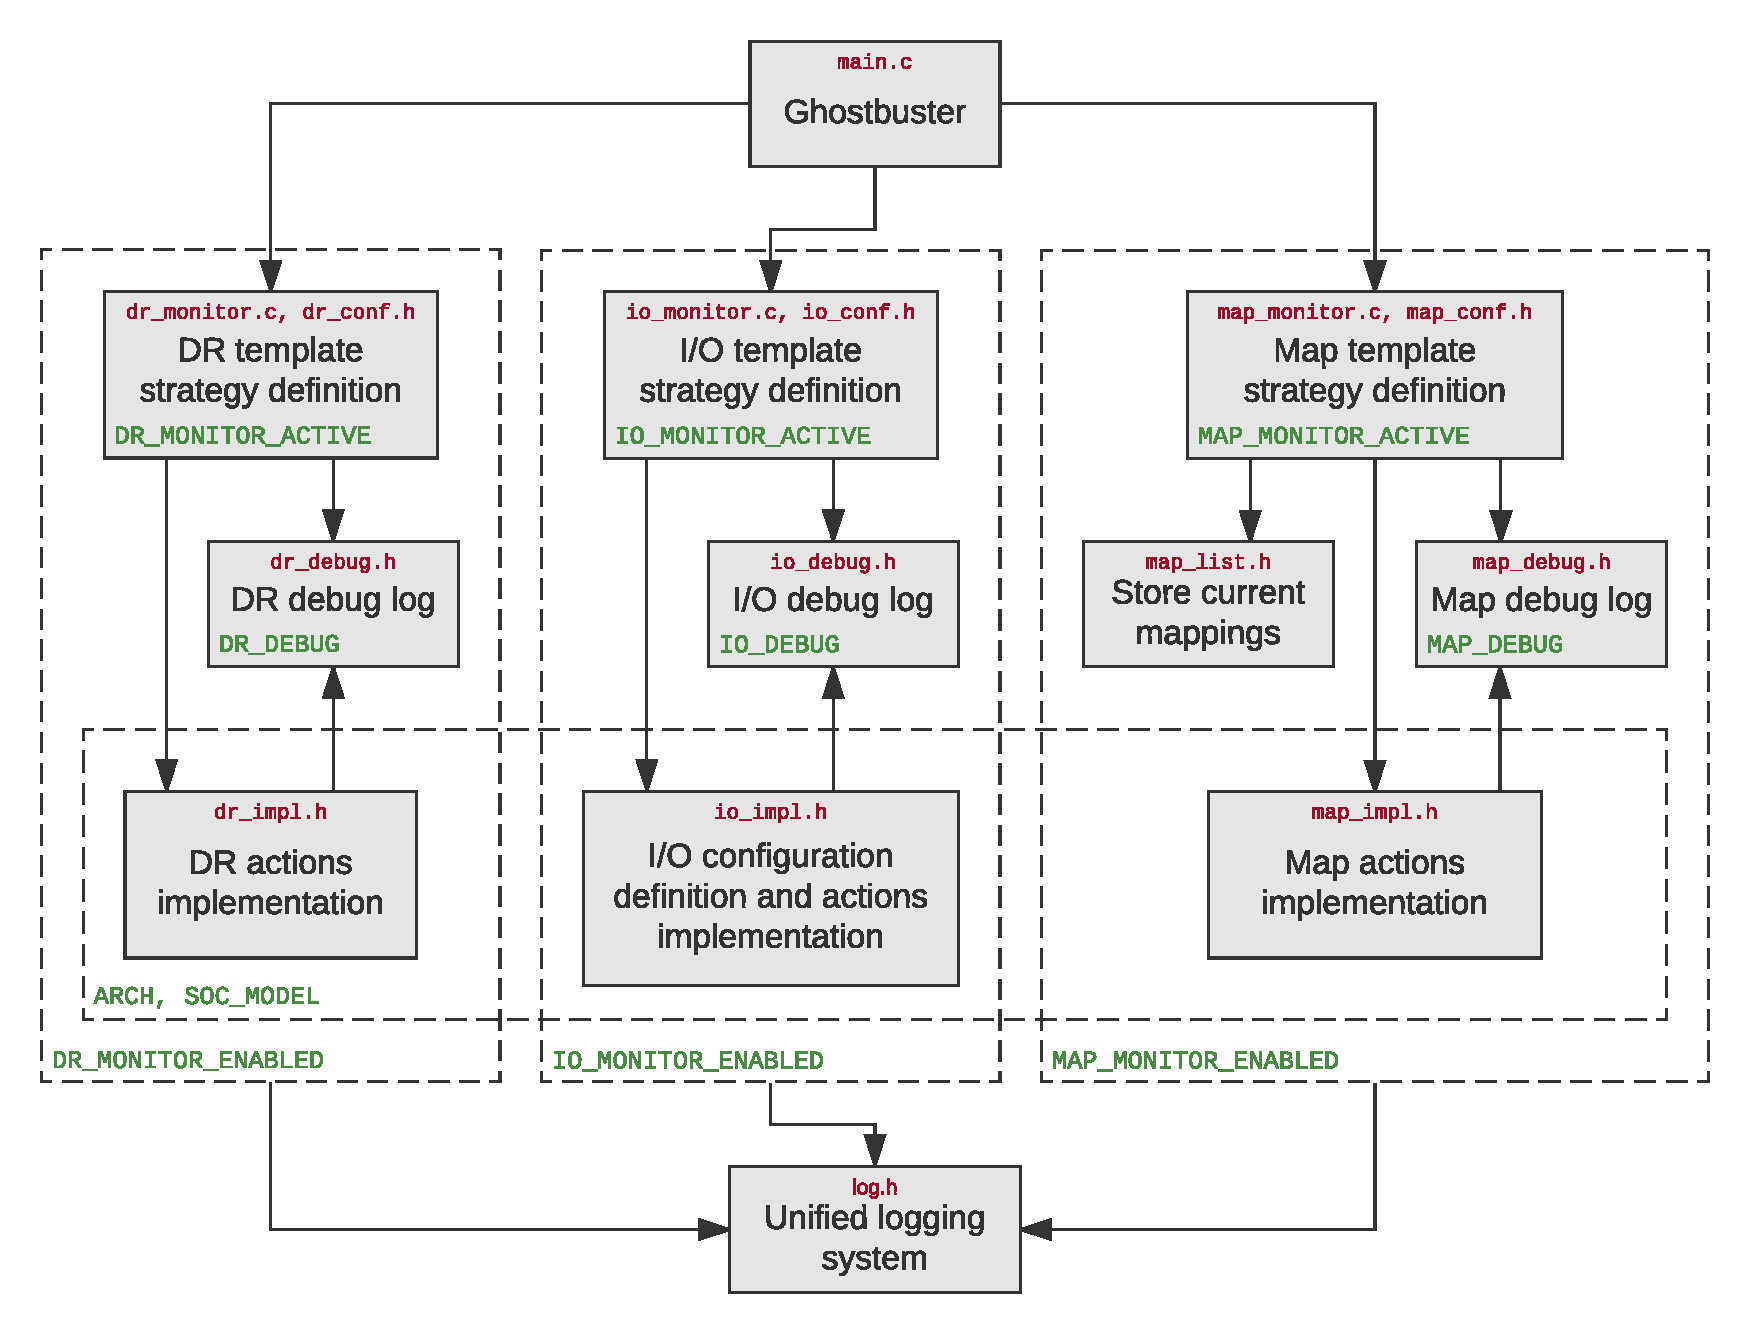
\includegraphics[width=\textwidth]{res/def-impl}}
\caption{Ghostbuster implementation architecture \label{fig:def-impl}}
\end{figure}
The resulting architecture is shown in \myfig{fig:def-impl}, which associates each specific role to the corresponding
source file(s) (in red).
Furthermore, the compilation of our module can be parameterised in different ways, as shown by the green labels in the figure.
Each green label, associated to a rectangle container in the figure, corresponds to a compiler flag that affects the compilation of the enclosed portion.
The compilation is managed by a \verb|Makefile|, in which all the required flags are defined.
The \verb|Makefile| needs to know the location of the target Linux kernel source directory.

In particular, each monitor can be enabled or disabled by means of the following flags:
\begin{Verbatim}[fontsize=\small]
	IO_MONITOR_ENABLED
	DR_MONITOR_ENABLED
	MAP_MONITOR_ENABLED
\end{Verbatim}
If a monitor is disabled, it will not be included into the compilation at all, reducing the final binary size.
This may be useful to exclude a particular monitor that is not needed by the target system
(\eg DR monitor if debug support is not enabled into the kernel, see discussion in \mysec{sec:dr-design}).

When a monitor is enabled, its execution mode may be controlled by one of the following flags, respectively:
\begin{Verbatim}[fontsize=\small]
	IO_MONITOR_ACTIVE
	DR_MONITOR_ACTIVE
	MAP_MONITOR_ACTIVE
\end{Verbatim}
If one of these flags is not defined, the corresponding monitor is compiled in \emph{passive} mode: it will only reports about events, without taking any further action.
Otherwise, the monitor is \emph{active} and it will include its specific reactions to the events.
If a monitor is disabled, the corresponding active flag is ignored.

The messages reported by each monitor may be extended by enabling the following debug flags:
\begin{Verbatim}[fontsize=\small]
	IO_DEBUG
	DR_DEBUG
	MAP_DEBUG
\end{Verbatim}
If a debug flag is defined, the corresponding monitor will print out its complete state at each event detection.

Finally, the \verb|ARCH| and \verb|SOC_MODEL| variables are used to select a specific implementation for the enabled monitors.
An implementation is identified by an architecture name and a SoC model (\eg \verb|arm|, \verb|BCM2835|). Given this information,
the implementation files will be automatically included from the \verb|<ARCH>/<SOC_MODEL>/| sub-directory.
We chose to directly include the implementation part into header files, instead of external compilation units (\verb|.c| files), to allow the usage of \verb|inline|
functions. The code of an inline function is directly included into the caller, and it does not need an explicit function call.
This may cause some code duplication, which we tried to minimise, but it achieves better performance,
especially for those functions that are called many times (\eg in the main loop of a monitor).

When Ghostbuster is loaded, the three main monitors are started in parallel.
The monitors are independent from each other, and every monitor has its own kernel thread.
When a monitor has to report an event to the system, it uses the common logging subsystem available into the kernel
(see \mysec{sec:def-usage} for more information).
The target systems used to test our defense are exactly the same as the ones described for the attack part in \mychap{chap:attack}, with the same PLC logic and I/O configuration.
In particular, for each monitor, we first refer to the Raspberry Pi system (BCM2835 SoC); then we discuss the modifications required to run on Wago PLC as well.
In the following sections we describe in more detail the structure and the operations performed by each monitor.
From now on, we will refer to the abstract part of each monitor as the \emph{interface}, and to the architecture-dependent part as the \emph{implementation}.


\subsection{I/O monitor}
\label{sec:io-impl}

This monitor is responsible for protecting I/O configuration memory from malicious usage.
The monitor interface includes the I/O configuration data type, modeled as a set of memory blocks by means of the \verb|io_conf_t| structure:
\begin{lstlisting}
typedef struct {
	const void** addrs; // Set of block base addresses
	const unsigned* sizes; // Size of each block in bytes
	const unsigned blocks; // Number of blocks
	const unsigned size; // Total size in byte
} io_conf_t;
\end{lstlisting}
This model takes into account the fact that I/O registers may be located at different addresses, resulting in a non-contiguous I/O memory.

With reference to the BCM2835 manual \cite{bcm2835} and to the target configuration defined in \mysec{sec:attack-pi},
we defined, into the implementation part, the set of I/O registers we want to protect.
In particular, since our system uses GPIO pins, two of which multiplexed to I2C, we chose to protect GPIO pin control registers, whose physical base address is \verb|0x2020000|.
These registers are responsible both for pin configuration and pin multiplexing. Each register is 32-bit wide, having 3 bits for each I/O pin: it can control $10$ different pins.
Although our target system uses only four pins for its I/O, to be more general, we decided to protect all the available GPIO pins ($54$).
Hence, we included all $6$ pin control registers into the definition of our I/O configuration, by filling in the \verb|io_conf_t| global structure:
\begin{lstlisting}
#define IO_BLOCKS            	1 // Registers are contiguous: one block needed
#define PIN_CTRL_BASE        	((void*)0x20200000) // Pin control base address
#define PIN_CTRL_SIZE        	24 // 6 regs * 4 bytes each
#define __IO_STATE_TOTAL_SIZE	24 // Total size in bytes

static const void* bcm2835_io_addrs[IO_BLOCKS] = { PIN_CTRL_BASE };
static const unsigned bcm2835_io_sizes[IO_BLOCKS] = { PIN_CTRL_SIZE };

static const io_conf_t phys_io_conf = {
	.addrs = bcm2835_io_addrs,
	.sizes = bcm2835_io_sizes,
	.blocks = IO_BLOCKS,
	.size = __IO_STATE_TOTAL_SIZE
};
\end{lstlisting}
Of course our implementation is only a prototype, and many other registers may be included into the I/O configuration (\eg event detect, edge detect, I2C control registers, etc.).

The next step is to define the trusted behaviour of the I/O configuration.
In particular, we have pin multiplexing (\emph{pinmux}) and pin configuration (\emph{pinconf}) registers, and we assumed the following behaviour:
\begin{itemize}
	\item \itemname{pinmux registers}: they are initialised at boot time, and never change during run-time;
	\item \itemname{pinconf registers}: they are initialised at boot time, but can be modified at any time by the PLC runtime, maintaining the following invariant:
		every pin configuration (input or output mode) must be conforming to the running PLC logic.
\end{itemize}

After I/O configuration has been defined, we can describe the interface and implementation of the I/O monitor.
The abstract part is essentially made of the monitor loop, which executes the main strategy,
and the detection handler, called by the implementation when an I/O modification has been detected. Both codes are shown in \myalg{alg:io-iface},
and they are independent from any specific architecture or SoC model.
\algnewcommand\True{\textbf{true}\space}
\algnewcommand\False{\textbf{false}\space}
\algnewcommand\algorithmicforeach{\textbf{for each}}
\algdef{S}[FOR]{ForEach}[1]{\algorithmicforeach\ #1\ \algorithmicdo}
\begin{algorithm}[h]
\caption{I/O monitor interface: main loop and detection handler}
\label{alg:io-iface}
\begin{algorithmic}[1]
\Function{IOMainLoop}{\null}
	\State $t \gets$ monitor scan interval \Comment{The monitor interval in $\SI{}{ms}$}
	\State $C \gets$ physical I/O configuration \Comment{The defined I/O configuration}
	\State $T \gets$ \Call{GetIOState}{$C$} \Comment{Read trusted state from I/O registers}
	\Loop
		\ForEach{block $B \in C$ having index $i$}
			\State \Call{CheckIOState}{$B, T[i]$} \Comment{Compare current and trusted state of block $B$}
		\EndFor
		\If{monitor should stop}
			\State \Return \Comment{Return if Ghostbuster is being stopped}
		\EndIf
		\State \Call{msleep}{$t$} \Comment{Wait for next cycle}
	\EndLoop
\EndFunction
\Statex
\end{algorithmic}

\begin{algorithmic}[1]
\Function{HandleIODetection}{$D$} \Comment{React to the detection $D$}
	\State report about D
	\If{I/O debug enabled}
		\State dump entire I/O state
	\EndIf
	\If{\Call{IsLegitimate}{$D$}}
		\State \Call{UpdateIOState}{$D$} \Comment{Accept new configuration, update trusted state}
	\Else
		\State report about Pin Control Attack
		\If{I/O monitor is active}
			\State \Call{RestoreIOState}{$D$} \Comment{Reject new configuration, restore trusted state back}
		\EndIf
	\EndIf
\EndFunction
\end{algorithmic}
\end{algorithm}

Each iteration of the main loop is executed every $t~\SI{}{ms}$, where the specific value of $t$ is defined into the \verb|IO_MONITOR_INTERVAL| flag.
The loop terminates only if an external signal indicates that Ghostbuster is being stopped (see \mysec{sec:def-usage}).
The verification of the current I/O configuration is performed at block level against the golden reference, which is obtained by \textproc{GetIOState} before starting the loop.
Since we assume that the system is in a safe state when our module is deployed, the initial I/O state read from configuration registers is considered trusted.
When a modification is detected by \textproc{CheckIOState}, the detection handler is called back and the monitor strategy is applied.
Note that the handler may be called many times from the same call to \textproc{CheckIOState}, because there may be more than one single modification within one contiguous block.
The detection granularity is decided by the implementation part (\eg for each single pin in our implementation).
If the modification is considered legitimate, then the reference I/O state is updated with the new configuration.
Otherwise, we report the attack to the system and, since we have an exact detection condition which cannot give false positives,
we may safely restore the previous configuration back if the I/O monitor is in active mode.

All the low-level I/O functions are defined into the implementation part, and may be different for each target system.
These functions deal with the effective accesses to I/O registers, which depend on many factors. The implementation knows the way to access these registers,
their size and their bits arrangement.
\begin{algorithm}[h!]
\caption{I/O monitor implementation functions}
\label{alg:io-impl}
\begin{algorithmic}[1]
\Function{GetIOState}{$C$} \Comment{Read current I/O state}
	\State $T \gets \emptyset$
	\ForEach{block $B$ in $C$}
		\ForEach{register $R \in B$}
			\State $T \gets T \cup \Call{ioread32}{$R$}$ \Comment{Save value of register $R$ into the trusted state}
		\EndFor
	\EndFor
	\State \Return $T$
\EndFunction
\Statex
\end{algorithmic}

\begin{algorithmic}[1]
\Function{CheckIOState}{$B, T_B$} \Comment{Verify block $B$ against its trusted state $T_B$}
	\ForEach{register $R \in B$ having index $i$}
		\State $C_R \gets \Call{ioread32}{$R$}$ \Comment{Read current value of register $R$}
		\State $T_R \gets T_B[i]$ \Comment{Trusted value of register $R$}
		\ForEach{pin $p \in R$ having index $j$}
			\State $d \gets C_R[j] \oplus T_R[j]$ \Comment{Difference between current and trusted value}
			\If{$d \neq 0$}
				\State $D \gets \{C_R, T_R, j, d\}$ \Comment{Fill in detection information}
				\State \Call{HandleIODetection}{$D$} \Comment{Call detection handler}
			\EndIf
		\EndFor
	\EndFor
\EndFunction
\Statex
\end{algorithmic}

\begin{algorithmic}[1]
\Function{IsLegitimate}{$D$}
	\If{$D$ is pin multiplexing}
		\State \Return false \Comment{Pin multiplexing is not allowed at run-time}
	\EndIf
	\If{$D$ is pin configuration}
		\If{new I/O configuration is conforming to PLC logic}
			\State \Return true \Comment{Change performed by the PLC runtime}
		\Else
			\State \Return false \Comment{Malicious change}
		\EndIf
	\EndIf
\EndFunction
\Statex
\end{algorithmic}

\begin{algorithmic}[1]
\Function{UpdateIOState}{$D$}
	\State $D.T_R[j] = D.C_R[j]$ \Comment{Update the trusted value according to new I/O configuration}
\EndFunction
\Statex
\end{algorithmic}

\begin{algorithmic}[1]
\Function{RestoreIOState}{$D$}
	\State \Call{iowrite32}{$D.T_R \oplus D.d$} \Comment{Restore I/O configuration to the trusted value}
\EndFunction
\end{algorithmic}
\end{algorithm}
In \myalg{alg:io-impl} we show our implementation related to the BCM2835 SoC, where all registers are 32-bits wide.

The detection events are managed at pin level, \ie if an attacker modifies the configuration of more than one pin at a time, only one pin at a time is verified.
The critical function of the implementation part is the \textproc{IsLegitimate} function, which decides whether a configuration change is legal or not.
Based on our behavioural model, pin multiplexing can never be legitimate during run-time, so the implementation is straightforward.
In the case of pin configuration, instead, the implementation needs to check if the I/O configuration after the change is in conflict with the PLC logic.
A conflict occurs in one of the following two cases:
\begin{itemize}
	\item \itemname{write}: the pin is set as input and the logic is trying to write from it;
	\item \itemname{read}: the pin is set as output and the logic is trying to read from it.
\end{itemize}
The most challenging problem here is to figure out which operation the logic is performing on a given I/O pin.
To solve this problem, we applied the reverse engineering approach proposed in \mysec{sec:io-design}, reported below. 

Inside the BCM2835, a specific set of 32-bit registers is used to interact with I/O pins: LVL registers to read the pin value,
CLR registers to write a $0$ and SET registers to write a $1$ \cite{bcm2835}. Every register contains a bit for each pin, for a total of 32 pins per register.
To have access to the operations performed by the PLC logic on these registers, we leveraged the debug subsystem.
In ARM architecture, the debug subsystem provides two different types of debug registers: breakpoint and watchpoint (see \mysec{sec:dr-impl}).
When a pin configuration change is detected, the I/O monitor inserts a watchpoint to the corresponding LVL, CLR or SET register of the affected pin,
in order to intercept the I/O operation performed by the PLC logic. The watchpoint can be set for either a read or a write, according to the specific case we want to verify.
From a reverse engineering analysis of the PLC runtime, we found that read and write operations are performed with the following instructions, respectively:
\begin{itemize}
	\item \verb|STR R2, [R3]| (Opcode \verb|0x002083E5|, \verb|R3| contains the address of a STR or CLR register);
	\item \verb|LDR R2, [R3]| (Opcode \verb|0x002093E5|, \verb|R3| contains the address of a LVL register).
\end{itemize}
\verb|R3| always contains the virtual address targeted by our watchpoint. When a watchpoint is hit, the debug exception handler is called,
and all the execution context of the process is passed as argument. Inside the debug handler, we proceed as follows, according to the case:
\begin{itemize}
	\item \itemname{write}: we look at the content of \verb|R2| to check if the PLC logic is trying to write to the specific pin changed to input.
		If \verb|R2| contains a $1$ corresponding to the target pin, then we can conclude that the new configuration is in conflict with the logic.
	\item \itemname{read}: in this case more reverse engineering of the PLC runtime is needed to know which pins (\ie bits) are actually used by the logic as input,
		because the instruction always loads the entire register (32 pins).
		To simplify the detection in our prototype version, we supposed that the PLC logic may only have one input pin for each register.
		In this case, reading from the register implies that the PLC logic is trying to read from the given pin. Thus, we can report a conflict.
		To remove this assumption, which limits the applicability of our defense, more knowledge about the PLC runtime is required.
		As previously discussed, this knowledge can be obtained either from a deeper reverse engineering analysis or from a collaboration with the PLC runtime vendor.
		For instance, each PLC logic may be designed to contain a constant bit mask having one bit for each pin,
		where each bit specifies whether the corresponding pin is currently used as input or output. If such data was available,
		the I/O monitor could look at it instead of inserting a watchpoint and looking for the actual operations.
		This mechanism raise the bar for the attacker, who would need to alter the PLC logic code as well to conduct the attack,
		thus defeating its stealthiness.
\end{itemize}

Note that from a performance perspective our approach is feasible, because it inserts a debug exception only in case of an I/O modification to determine if it is malicious.
Thus, this may cause an overhead when a good I/O configuration is updated by the PLC runtime as well. See \mychap{chap:results} for more details about our results.

Besides its main functions, the I/O monitor provides an additional interface, which is needed by the MAP monitor.
When the MAP monitor has to filter mapping requests coming from system processes, it needs to know whether a request of a physical address range includes
at least one address belonging to the I/O configuration. This is provided by the I/O monitor with the function listed in \myalg{alg:io-overlap},
which accepts a pair of physical addresses $[s, e]$ representing the start and the end addresses of the given range.
\begin{algorithm}[h]
\caption{I/O monitor overlap function}
\label{alg:io-overlap}
\begin{algorithmic}[1]
\Function{MapOverlapsIO}{$s, e$} \Comment{Check if physical range $[s, e]$ overlaps I/O configuration}
	\State $C \gets$ physical I/O configuration \Comment{The defined I/O configuration}
	\ForEach{block $B$ in $C$}
		\If{$(B.s \le s \le B.e) \lor (B.s \le e \le B.e)$} \Comment{Overlap condition at block level}
			\State \Return \True
		\EndIf
	\EndFor
	\State \Return \False
\EndFunction
\end{algorithmic}
\end{algorithm}
Since this function is needed by the MAP monitor independently from I/O monitor operations, we designed it to be available even if the I/O monitor is disabled.
The I/O configuration, needed by \textproc{MapOverlapsIO}, is made available independently from the I/O monitor as well.
Note that, there might exist some target systems in which disabling the I/O monitor has sense. For instance, consider a system having the following two properties:
\begin{itemize}
	\item the root/kernel access is properly protected (\eg kernel protected by execute only memory or TrustZone),
		or it has sufficient security level for which is not worth to insert the I/O monitor (\eg no admin default passwords, hardened kernel, etc.);
	\item the PLC runtime, or any other process, does not use the mapping interface (\ie on Wago PLC).
\end{itemize}
On such a system, the MAP monitor alone could be enough to protect the I/O configuration, because it can simply deny any access to I/O physical addresses from user space,
while the system itself is already protected from kernel space accesses.


\subsubsection{Wago PLC version}

To port the I/O monitor to the Wago PLC system, only the following changes are necessary:
\begin{itemize}
	\item \itemname{I/O configuration}: the I/O configuration and the behavioural model must be redefined according to the registers used by the Wago PLC.
		In particular, the implementation may include pin configuration and pin multiplexing registers as well, plus SPI, DMA and IRQ registers.
		The way to access registers is pretty much equal to the Raspberry Pi system, because are both ARM architectures with 32-bit wide registers.
		On Wago PLC, pin configuration and pin multiplexing are managed by two different set of registers. Therefore, the low-level implementation
		is even simplified, because it does not need to distinguish configuration and multiplexing bits inside registers.
		However, including other registers (\eg SPI, DMA, IRQ, etc.) may lead to more complex behavioural models which need to be analysed.
	\item \itemname{Debug subsystem}: given the engineering problem described later in \mysec{sec:dr-impl}, the same solution using watchpoint cannot be directly applied.
		To get the needed information about the PLC logic, two ways are possible. Either the debug interface is implemented into the kernel for AM3517 SoC,
		or a better integration with the PLC runtime is required, as already discussed.
\end{itemize}


\subsection{DR monitor}
\label{sec:dr-impl}

The DR monitor aims to protect the debug subsystem. As described for the design phase, the DR monitor needs to accomplish two goals:
\begin{itemize}
	\item disable debug interface access from user space;
	\item watch over debug registers value to detect malicious events.
\end{itemize}

In Linux, the debug user interface is based on the following functions \cite{hw-breakpoint}:
\begin{lstlisting}
struct perf_event* register_user_hw_breakpoint(struct perf_event_attr* attr,
                                               perf_overflow_handler_t handler,
                                               struct task_struct* tsk);

int modify_user_hw_breakpoint(struct perf_event *bp,
                              struct perf_event_attr *attr);

void unregister_hw_breakpoint(struct perf_event *bp);
\end{lstlisting}
To disable these functions, we dynamically patched the kernel text replacing the prologue instructions of each function.
In particular, they have the following prologue:
\begin{Verbatim}[fontsize=\small]
	c00d3cb0 <register_user_hw_breakpoint>:
	c00d3cb0: e1a0c00d  mov  ip, sp
	c00d3cb4: e92dd800  push {fp, ip, lr, pc}
	c00d3cb8: e24cb004  sub  fp, ip, #4
	c00d3cbc: e24dd008  sub  sp, sp, #8
	[...]

	c00d3e30 <modify_user_hw_breakpoint>:                                
	c00d3e30: e1a0c00d  mov  ip, sp
	c00d3e34: e92ddff0  push {r4, r5, r6, r7, r8, r9, sl, fp, ip, lr, pc}
	c00d3e38: e24cb004  sub  fp, ip, #4
	c00d3e3c: e24dd00c  sub  sp, sp, #12
	[...]

	c00d3ce8 <unregister_hw_breakpoint>:
	c00d3ce8: e1a0c00d  mov   ip, sp
	c00d3cec: e92dd800  push  {fp, ip, lr, pc}
	c00d3cf0: e24cb004  sub   fp, ip, #4
	[...]
\end{Verbatim}
We replaced the prologue instructions with the following ones:
\begin{enumerate}
	\item \itemname{return value}: if the function is not void (\eg in the first two cases), we need to return a value to the caller.
		Thus, we move the value \verb|-EACCES| ($-13$) into R0 by using the move-negate instruction: \verb|mvn r0, #0xC|.
		\verb|EACCES| is defined into the \verb|errno-base.h| kernel header as \verb|Permission denied|;
	\item \itemname{branch}: jump back to the caller by branching to the link register: \verb|bx lr|.
\end{enumerate}
After the patch, the kernel text becomes the following:
\begin{Verbatim}[fontsize=\small]
	c00d3cb0 <register_user_hw_breakpoint>:
	c00d3cb0: e3e0000c  mvn  r0, #0xC
	c00d3cb4: e12fff1e  bx   lr
	[...]

	c00d3e30 <modify_user_hw_breakpoint>:                                
	c00d3e30: e3e0000c  mvn  r0, #0xC
	c00d3e34: e12fff1e  bx   lr
	[...]

	c00d3ce8 <unregister_hw_breakpoint>:
	c00d3ce8: e12fff1e  bx   lr
	[...]
\end{Verbatim}

Once the user access to debug registers has been disabled, we activate the DR monitor to protect them from attackers who gain kernel access.
As for the I/O monitor, we report the interface part and the implementation.
The abstract strategy of the DR monitor is rather simple, and is listed in \myalg{alg:dr-iface}.
\begin{algorithm}[h]
\caption{DR monitor interface: main loop and detection handler}
\label{alg:dr-iface}
\begin{algorithmic}[1]
\Function{DRMainLoop}{\null}
	\State $m_T \gets$ mutex \Comment{Global mutex to protect trusted state}
	\State $t \gets$ monitor scan interval \Comment{The monitor interval in $\SI{}{ms}$}
	\State $T \gets$ \Call{GetDRState}{\null} \Comment{Read trusted state from debug registers}
	\Loop
		\State \Call{lock}{$m_T$}
		\State \Call{CheckDRState}{$T$} \Comment{Compare current and trusted state of debug registers}
		\State \Call{unlock}{$m_T$}
		\If{monitor should stop}
			\State \Return \Comment{Return if Ghostbuster is being stopped}
		\EndIf
		\State \Call{msleep}{$t$} \Comment{Wait for next cycle}
	\EndLoop
\EndFunction
\Statex
\end{algorithmic}

\begin{algorithmic}[1]
\Function{HandleDRDetection}{$D$} \Comment{React to the detection $D$}
	\If{DR debug enabled}
		\State dump entire DR state
	\EndIf
	\State report about Pin Control Attack
	\If{DR monitor is active}
		\State \Call{RestoreDRState}{$D$} \Comment{Restore debug register trusted state}
	\EndIf
\EndFunction
\end{algorithmic}
\end{algorithm}
It is a simplification of the I/O monitor strategy, where any modification is considered malicious.
Since in our implementation the I/O monitor makes use of the debug subsystem, the DR monitor exposes the interface listed in \myalg{alg:dr-ioiface}
to mediate any access to debug registers.
\begin{algorithm}[h]
\caption{DR monitor interface for I/O monitor}
\label{alg:dr-ioiface}
\begin{algorithmic}[1]
\Function{SetDR}{$r$} \Comment{Set a debug register $r$}
	\State \Call{lock}{$m_T$}
	\State \Call{register\_wide\_hw\_breakpoint}{$r$} \Comment{Use kernel interface for debug registers}
	\State $T \gets$ \Call{GetDRState}{\null} \Comment{Update trusted state}
	\State \Call{unlock}{$m_T$}
\EndFunction
\Statex
\end{algorithmic}

\begin{algorithmic}[1]
\Function{ResetDR}{$r$} \Comment{Reset a previously set debug register $r$}
	\State \Call{lock}{$m_T$}
	\State \Call{unregister\_wide\_hw\_breakpoint}{$r$} \Comment{Use kernel interface for debug registers}
	\State $T \gets$ \Call{GetDRState}{\null} \Comment{Update trusted state}
	\State \Call{unlock}{$m_T$}
\EndFunction
\end{algorithmic}
\end{algorithm}
By using this interface, any modification of debug registers performed by the I/O monitor is excluded from the detection.
This mechanism requires that the DR state is protected from concurrent access by a mutual exclusion mechanism.
%the interface is usable by the attacker?

All the details about debug registers are handled by the implementation part, shown in \myalg{alg:dr-impl}.
\begin{algorithm}[h]
\caption{DR monitor implementation functions}
\label{alg:dr-impl}
\begin{algorithmic}[1]
\Function{GetDRState}{\null} \Comment{Read current I/O state}
	\State $T \gets \emptyset$
	\State $D \gets hardware debug registers$
	\ForEach{debug register $r \in D$}
		\State $T \gets T \cup \Call{DRread}{$r$}$ \Comment{Save value of debug register $r$ into $T$}
	\EndFor
	\State \Return $T$
\EndFunction
\Statex
\end{algorithmic}

\begin{algorithmic}[1]
\Function{CheckDRState}{$T$} \Comment{Verify debug registers against trusted state $T_B$}
	\ForEach{debug register $r \in B$ having index $i$}
		\State $C_r \gets \Call{DRread}{$r$}$ \Comment{Read current value of register $r$}
		\State $T_r \gets T[i]$ \Comment{Trusted value of register $r$}
		\State $d \gets C_r \oplus T_r$ \Comment{Difference between current and trusted value}
		\If{$d \neq 0$}
			\State $D \gets \{C_r, T_r, r\}$ \Comment{Fill in detection information}
			\State \Call{HandleDRDetection}{$D$} \Comment{Call detection handler}
		\EndIf
	\EndFor
\EndFunction
\Statex
\end{algorithmic}

\begin{algorithmic}[1]
\Function{RestoreDRState}{$D$}
	\State \Call{DRwrite}{$D.r, D.T_r$} \Comment{Restore debug register to the trusted value}
\EndFunction
\end{algorithmic}
\end{algorithm}
The ARM architecture supports two type of hardware debug registers: breakpoints for instruction addresses, and watchpoints for data addresses.
The DR monitor protects both of them, and the detection is handled at register level. Each register is accessed through specific coprocessor instructions.
A special read-only register, the \emph{Debug ID Register} (DIDR), specifies the number of debug registers available and other useful information on the SoC configuration.
In particular, since the BCM2835 SoC supports 2 watchpoints and 6 breakpoints, the DR monitor can be deployed to protect them all.


\subsubsection{Wago PLC version}

To adapt the DR monitor for Wago PLC, the following engineering problem needs to be solved.
The AM3517 SoC model embedded into this PLC provides a different interface for debug registers. In particular, it uses a memory mapped interface
instead of specific coprocessor instructions \cite{am35x}.
Unfortunately, it turns out that this particular interface is not supported by the Linux kernel debug framework, as reported in \cite{dr-mapped}:
``The memory-mapped extended debug interface is unsupported due to its unreliability in real implementations''.
Apart from this technical problem, the DR monitor is designed to be applicable to any other ARM implementation that supports debug registers.
To port it for other architectures different than ARM, only the implementation part must be adapted.


\subsection{MAP monitor}
\label{sec:map-impl}

The purpose of the MAP monitor is to filter user space requests delivered to the mapping subsystem. On Linux, users can use the mapping interface to
map files or devices, and this mechanism can be used to map physical addresses to virtual addresses through special devices such as \verb|/dev/mem|.
Among all physical memory addresses, an attacker may be able to map specific I/O memory regions to alter I/O configuration registers.
The set of devices that can provide access to I/O physical memory depends on the specific system
(\eg for the Linux version installed on our Raspberry Pi, either \verb|/dev/mem| or \verb|/dev/gpiomem| can be used).
Linux provides the following system calls to deal with mapping requests:
\begin{lstlisting}
long mmap2(unsigned long addr, unsigned long len,
           unsigned long prot, unsigned long flags,
           unsigned long fd, unsigned long pgoff);

long mremap(unsigned long addr,
            unsigned long old_len, unsigned long new_len,
            unsigned long flags, unsigned long new_addr);

long remap_file_pages(unsigned long addr, unsigned long len,
                      unsigned long prot, unsigned long pgoff,
                      unsigned long flags);

long munmap(unsigned long addr, size_t len);
\end{lstlisting}
Note that we are describing the interface from a kernel point of view: the interface exposed to user space may be slightly different.
The \verb|mmap2| system call supersedes the old \verb|mmap|, and both use the same internal function which is \verb|sys_mmap_pgoff|.
Although these functions are used for many other types of mappings, we focus on mappings between virtual addresses and physical memory addresses.
These system calls serve the following purpose, respectively:
\begin{itemize}
	\item \itemname{mmap2}: request a new mapping related to the \verb|fd| address space (\eg \verb|/dev/mem| for physical memory) having \verb|len| bytes
		and starting from page offset \verb|pgoff|; returns the mapped virtual address pointing to the starting offset of the target address space;
	\item \itemname{mremap}: modify an existing mapping, either remapping it to a new virtual address \verb|new_addr| (\emph{move})
		or resizing it to \verb|new_len| bytes (\emph{grow} or \emph{shrink}); returns the virtual address after the modification;
	\item \itemname{remap\_file\_pages}: remap an existing mapping to point to a different start page offset \verb|pgoff| of the target address space
		(\eg to point to a different physical address); returns $0$ if successful, an error code otherwise.
	\item \itemname{munmap}: delete an existing mapping of \verb|len| bytes related to the virtual address \verb|addr|;
		the \verb|len| parameter is aligned to the next page boundary, and the resulting range of pages is removed.
\end{itemize}
The type of a requested mapping can be inferred from the \verb|fd| (file descriptor) parameter in \verb|mmap2|,
or from the \verb|addr| parameter in the other calls, which refer to previously mapped regions.
Every mapping is managed at a page level, and the arguments are aligned to page boundaries before handling the request.
The scheme in \myfig{fig:map-linux} summarises a significant sequence of operations performed via the mapping interface,
assuming physical and virtual address spaces based on $\SI{4}{\kilo\byte}$ pages.
\begin{figure}[h]
\centerline{
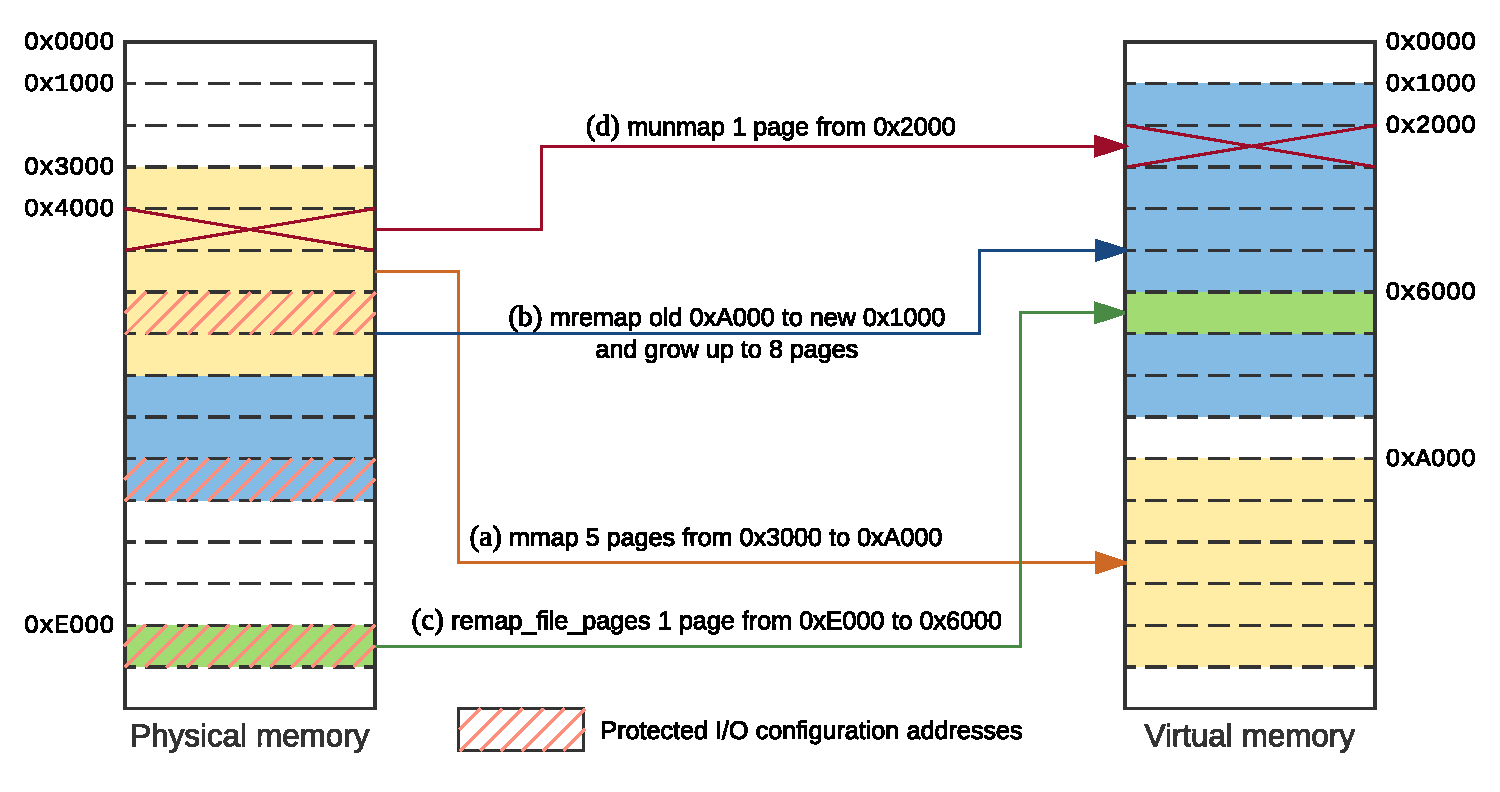
\includegraphics[width=\textwidth]{res/map-linux}}
\caption{Accessing physical addresses through Linux mapping interface \label{fig:map-linux}}
{\phantomsubcaption\ignorespaces\label{fig:mmap}}
{\phantomsubcaption\ignorespaces\label{fig:mremap}}
{\phantomsubcaption\ignorespaces\label{fig:remapfp}}
{\phantomsubcaption\ignorespaces\label{fig:munmap}}
\end{figure}
As shown in the figure, there exist $3$ different ways of accessing protected I/O physical addresses by using mapping functions.
When a mapping includes a portion (even one byte) of the I/O configuration defined by the I/O monitor, we say that an \emph{overlap} occurs.
First, an attacker may call \verb|mmap2| (or \verb|mmap|) to directly include the I/O configuration into the requested range \subref{fig:mmap}.
Second, he may use \verb|mremap| to extend a current mapping, possibly causing overlap on an I/O address which was not mapped before \subref{fig:mremap}.
Third, he can re-map an already mapped virtual address to a different physical address, including a protected I/O address as well \subref{fig:remapfp}.
Note that, the second and the third system calls identify the existing mappings by means of the virtual addresses returned by the first call to \verb|mmap2|.
Therefore, the MAP monitor must keep track of the current existing mapping (and virtual addresses) to verify if a subsequent re-map may cause an overlapping.
Finally, the \verb|munmap| call deletes an existing mapping (or part of it) \subref{fig:munmap}. Even if it cannot cause an overlap,
the \verb|munmap| system call needs to be monitored as well in order to update the data structure containing the existing mappings and remain
consistent with the kernel data structures.

To keep track of the current mappings related to physical memory, our monitor uses a global list of pages. Each page is a structure containing a physical address,
a virtual address, and a process identifier. We assume that the number of processes normally interested in physical memory is quite low.
Hence, a global list containing mapped pages of all the processes together performs well enough for our purpose.
If that is not the case, the monitor could be improved, \eg by using a hash-table based on process identifiers.
The definition of our data structure, which uses the list defined into the \verb|<list.h>| kernel header, is reported below:
\begin{lstlisting}
typedef struct {
	struct list_head pages; // Pointer to the rest of the list
	unsigned long paddr; // The page physical address
	unsigned long vaddr; // The page virtual address
	pid_t pid; // The process who requested the mapping
} page;
LIST_HEAD(page_list); // The list head
DEFINE_MUTEX(page_list_lock); // To protect the list from concurrent accesses
\end{lstlisting}
Since the mapping system calls may be called by different processes concurrently, our data structure needs to be protected by a mutual exclusion mechanism.
The implementation supports classical operations such as insert, search, update and remove, each one at a page level.

The abstract part of our monitor is basically made of $4$ hook functions having the same prototype of the system calls described above.
These functions replace the original system calls, to receive all the mapping requests coming from user space.
When a map request is not interesting (\eg does not target physical memory) or it is allowed, the monitor forwards the request to the original system call.
Otherwise, the monitor policy is applied, and the request may be denied before reaching the original system call.
Our approach is feasible because does not use slow mechanisms such as kprobes \cite{kprobes}, but it directly replaces the pointers into the system call table.
Note that this mechanism is just a prototype, and it has some minor drawbacks that could be reduced. For instance, since our functions must be consistent
with the original system calls, some code needs to be duplicated. In particular, we need to check the arguments used by the monitor in the same way the original system calls do
(\eg for page alignment). This could be avoided by including our monitor as part of the kernel code itself. Note that this improvement may be worth considering that
the mapping system calls might be called many times during run-time, since they are not only used for physical memory but for any file/device mapping.

The abstract part of the MAP monitor, shown in \myalg{alg:map-iface}, is independent from the specific architecture.
It makes use of the \textproc{AddMapping}, \textproc{GetMappingPhysAddr}, \textproc{UpdateMapping}, \textproc{AlterMapping} and \textproc{DeleteMapping}
functions provided by the page list structure. We omit their implementation because it is straightforward and does not add anything to our discussion.
\textproc{PageAlign} (and \textproc{PageMask}), \textproc{PageShift} and \textproc{error}, instead, refer to corresponding Linux kernel macros that deal with
page alignment, page offset and error handling, respectively.
For system calls that do not have the file descriptor as parameter, to check if a request refers to a physical memory mapping, and not to other files/devices,
we look into our page list.
\begin{algorithm}[h]
\caption{MAP monitor interface: hook functions for mapping system calls}
\label{alg:map-iface}
\begin{algorithmic}[1]
\Function{MyMmap}{$addr, len, prot, flags, fd, pgoff$} \Comment{mmap (mmap2) hook}
	\State $pid \gets$ current pid
	\State $len \gets \Call{PageAlign}{len}$ \Comment{Align len to next page boundary}
	\If{\Call{IsPhysMem}{$fd$}} \Comment{If it is a physical memory mapping}
		\State $s \gets \Call{PageShift}{pgoff}$ \Comment{Start physical address}
		\State $e \gets s + len$ \Comment{End physical address}
		\If{\Call{MapOverlapsIO}{$s, e$}} \Comment{Use I/O monitor interface}
			\State report about overlap
			\If{monitor is active}
				\State \Return $-13$ \Comment{Permission denied}
			\EndIf
		\EndIf
		\State $r \gets \Call{mmap2}{addr, len, prot, flags, fd, pgoff}$ \Comment{Original system call}
		\If{$\neg \Call{error}{r}$} \Comment{Call succeeded}
			\State \Call{AddMapping}{$s, e, r, pid$} \Comment{Add mapped pages to the page list}
		\EndIf
		\State \Return $r$
	\EndIf
	\State \Return \Call{mmap2}{$addr, len, prot, flags, fd, pgoff$} \Comment{Original system call}
\EndFunction
\Statex
\end{algorithmic}

\begin{algorithmic}[1]
\Function{MyMremap}{$addr, oldLen, newLen, flags, newAddr$} \Comment{mremap hook}
	\If{$addr$ is not page aligned} \Comment{mremap requires a page aligned address}
		\State \Return \Call{mremap}{$addr, oldLen, newLen, flags, newAddr$} \Comment{It will fail}
	\EndIf
	\State $pid \gets$ current pid
	\State $oldLen \gets \Call{PageAlign}{oldLen}$ \Comment{Align old length to next page boundary}
	\State $newLen \gets \Call{PageAlign}{newLen}$ \Comment{Align new length to next page boundary}
	\State $s \gets \Call{GetMappingPhysAddr}{addr, pid}$ \Comment{Search page list for start physical address}
	\If{$\neg \Call{error}{s}$} \Comment{If it is a physical memory mapping}
		\If{$newLen > oldLen$} \Comment{Growing is dangerous}
			\State $e \gets s + newLen$ \Comment{End physical address}
			\If{\Call{MapOverlapsIO}{$s, e$}} \Comment{Use I/O monitor interface}
				\State report about overlap
				\If{monitor is active}
					\State \Return $-13$ \Comment{Permission denied}
				\EndIf
			\EndIf
		\EndIf
		\State $r \gets \Call{mremap}{addr, oldLen, newLen, flags, newAddr}$ \Comment{Original system call} 
		\If{$\neg \Call{error}{r}$} \Comment{Call succeeded}
			\State \Call{UpdateMapping}{$addr, oldLen, r, newLen, s, pid$} \Comment{Update pages in page list}
		\EndIf
		\State \Return $r$
	\EndIf
	\State \Return \Call{mremap}{$addr, oldLen, newLen, flags, newAddr$} \Comment{Original system call}
\EndFunction
\end{algorithmic}
\end{algorithm}
\begin{algorithm}[h]
\ContinuedFloat
\begin{algorithmic}[1]
\Function{MyRemapFilePages}{$addr, len, prot, pgoff, flags$} \Comment{remap\_file\_pages hook}
	\State $addr \gets \Call{PageMask}{addr}$ \Comment{Align addr to previous page boundary}
	\State $len \gets \Call{PageAlign}{len}$ \Comment{Align len to next page boundary}
	\State $s \gets \Call{GetMappingPhysAddr}{addr, pid}$ \Comment{Search page list for start physical address}
	\If{$\neg \Call{error}{s}$} \Comment{If it is a physical memory mapping}
		\State $s \gets \Call{PageShift}{pgoff}$ \Comment{Start physical address}
		\State $e \gets s + len$ \Comment{End physical address}
		\If{\Call{MapOverlapsIO}{$s, e$}} \Comment{Use I/O monitor interface}
			\State report about overlap
			\If{monitor is active}
				\State \Return $-13$ \Comment{Permission denied}
			\EndIf
		\EndIf
		\State $r \gets \Call{remap\_file\_pages}{addr, len, prot, pgoff, flags}$ \Comment{Original system call} 
		\If{$r == 0$} \Comment{Call succeeded}
			\State \Call{AlterMapping}{$addr, s, len, pid$} \Comment{Update pages in page list}
		\EndIf
		\State \Return $r$
	\EndIf
	\State \Return \Call{remap\_file\_pages}{$addr, len, prot, pgoff, flags$} \Comment{Original system call}
\EndFunction
\Statex
\end{algorithmic}

\begin{algorithmic}[1]
\Function{MyMunmap}{$addr, len$} \Comment{munmap hook}
	\If{$addr$ is not page aligned} \Comment{munmap requires a page aligned address}
		\State \Return \Call{munmap}{$addr, len$} \Comment{It will fail}
	\EndIf
	\State $s \gets \Call{GetMappingPhysAddr}{addr, pid}$ \Comment{Search page list for start physical address}
	\If{$\neg \Call{error}{s}$} \Comment{If it is a physical memory mapping}
		\State report about $s$ being unmapped
		\State \Call{DeleteMapping}{$addr, len, pid$} \Comment{Delete pages from page list}
	\EndIf
	\State \Return \Call{munmap}{$addr, len$} \Comment{Original system call}
\EndFunction
\end{algorithmic}
\end{algorithm}
If the given virtual address \verb|addr| is not mapped into the list by the current \verb|pid|, \ie it does not map a valid physical address,
then two possibilities exist. Either the virtual address is mapped to some other device (not included into the list by our mmap hook), or the process is sending
a bad virtual address. In both cases we are not interested to the request, and we can let the original system call manage it.

The implementation part of the MAP monitor deals with the actual hooking procedure, which includes the following operations:
\begin{enumerate}
	\item finding the system call table base address in kernel memory;
	\item storing a copy of the original system call pointers to allow the abstract part to call them when necessary;
	\item replacing them with pointers to the hook functions defined above.
\end{enumerate}
Several technical details of these operations, which we omit in this report, depend on the actual architecture
(\eg find system call table, page write attribute, size of pointers, system call convention, etc.).
The interesting part of the implementation is the function responsible for identifying whether a map request refers to physical memory or not.
This is also dependent from the particular target system.
For instance, the code listed below is related to the \textproc{IsPhysMem} implementation for our Raspberry Pi system:
\begin{lstlisting}
static inline int is_phys_mem(unsigned long fd) {
	int res = NOT_PHYS_MEM;
	struct file *f = fget(fd);
	if (!f) goto bad_fd;
	if (f->f_op->mmap == mmap_mem) // mmap request for physical memory
		res = PHYS_MEM;
	fput(f);
bad_fd:
	return res;
}
\end{lstlisting}
where \verb|mmap_mem| points to the kernel function which handles the requests for \verb|/dev/mem|:
\begin{lstlisting}
mmap_mem = (void*)kallsyms_lookup_name("mmap_mem");
\end{lstlisting}

Since in our target system the PLC runtime requests a new mapping from user space every time a PLC logic is uploaded,
we configured the monitor as passive, to only report the mapping requests. Thus, it only provides additional information about an eventual attack from user space.
This could be improved by providing reports based on a statistical model of the PLC runtime requests, or even better by designing a defense-aware PLC runtime.
For instance, if our detection mechanism is integrated with the PLC runtime as described later in \mysec{sec:def-usage}, the MAP monitor may be used in the following way:
\begin{itemize}
	\item when a new mapping request has been detected, Ghostbuster can signal the PLC runtime;
	\item the PLC runtime knows if the request is due to a current logic update; if it is not, the runtime can rethrow the alert to the operator terminal.
\end{itemize}
The optimal solution, of course, would be to completely avoid using mapped I/O addresses from user space, and manage the I/O from kernel space only.
However, depending on the actual implementation, this could require several changes in the PLC software. Therefore, using the signaling approach might be preferred in that case.


\subsubsection{Wago PLC version}

On Wago PLC system, the I/O is entirely managed from kernel space already, and from our experiments we found that no user processes send mapping requests for physical memory.
Thus, the MAP monitor can be configured as active, to directly deny any I/O map request from user space.
Since this PLC is based on ARM architecture as well, the MAP monitor does not need any modification to be ported to this system,
except for the \verb|is_phys_mem| function that should target only the \verb|/dev/mem| device (\verb|/dev/gpiomem| only exists on Raspberry Pi).
Therefore, for Wago PLC, the MAP monitor alone can actually prevent any attack residing in user space, because the operating system does not provide
any other mechanism for users to access physical memory.


\subsection{Module usage}
\label{sec:def-usage}

Our defense can be either dynamically inserted as a Loadable Kernel Module (LKM), or can be built-in into the Linux kernel.
The second approach requires a kernel re-compilation to obtain a new kernel image including our module.
There are no performance differences between the two configurations, the only difference is that if an LKM is used, it can be unloaded as well.
The security implications of these two approaches are discussed in \mysec{sec:def-sec}.

In our prototype version for Raspberry Pi, the I/O monitor needs to set a watchpoint on a PLC runtime virtual address to verify the I/O configuration
against the current I/O operations. Therefore, we need to pass this virtual address as parameter, together with the process identifier of the PLC runtime, to our kernel module.
This could be avoided by a better integration between our module and the PLC runtime.
For instance, it could be the Ghostbuster module itself to start the PLC runtime process and provide the mapped virtual address.

After building the module, it can be loaded by means of the following Bash script that looks for pid and I/O base virtual address of the PLC runtime:
\begin{lstlisting}[language=bash]
#!/bin/sh
ppid=`pidof codesyscontrol.bin | cut -d' ' -f 1`
vaddr=`cat /proc/$ppid/maps | grep /dev/mem | cut -d'-' -f 1 | cut -d' ' -f 1`

insmod ghostbuster.ko p_pid=$ppid vaddr_base=0x$vaddr
if [ $? = 0 ]
then
	echo "Loading Ghostbuster... done!"
else
	echo "Loading Ghostbuster... failed!"
fi
\end{lstlisting}

When the module is running, all the information about detection events is reported among the other kernel messages, accessible by the \verb|dmesg| tool as follows:
\begin{Verbatim}
  root@raspberrypi:~ # dmesg -T
  [Tue Nov 15 10:54:42 2016] Ghostbuster: I/O monitor started
  [Tue Nov 15 10:54:42 2016] Ghostbuster: DR monitor started
  [Tue Nov 15 10:54:42 2016] Ghostbuster: MAP monitor started
  [Tue Nov 15 10:54:42 2016] Ghostbuster: Ghostbuster started
  [Tue Nov 15 10:55:50 2016] [RK] init
  [Tue Nov 15 10:55:50 2016] [RK] Pin Multiplexing Hijacked!
  [Tue Nov 15 10:55:50 2016] Ghostbuster: I/O change detected:
	phys[0xf2200000] [old value = 0x00048924, new value = 0x00048824]
  [Tue Nov 15 10:55:50 2016] Ghostbuster: Illegal change: Pin Control Attack!
  [Tue Nov 15 10:55:50 2016] Ghostbuster: I/O state restored
\end{Verbatim}
In the code above, the kernel module variant of Pin Control Attack (\verb|RK|) has been immediately detected by Ghostbuster.
In the current implementation, the reporting mechanism is just a prototype that prints messages only useful for testing and logging.
In a final version, a mechanism to send alarm signals to the PLC runtime should be implemented.
Then, the runtime itself must be designed to handle and report these signals to a connected terminal as well,
to allow the industrial operator to analyse the report and take further countermeasures according to the industrial policies.


\section{Security considerations}
\label{sec:def-sec}

Our detection system has been designed having in mind the threat model in \mysec{sec:threat-model} as well as the attack implementations presented in \mysec{sec:attack-impl}.
The design is meant to be as much general as possible, since it aims to cover different attack vectors and to be applicable
on several target systems that may be heterogeneous in their characteristics.
The definition of the monitor strategies and policies is a key aspect for having a significant solution that raises the bar for the attacker.

In our work we assumed that the system is protected from classical function and data hooking techniques, as it will likely be in the next years.
In this scenario, malicious users will be forced to avoid these techniques, and to leverage lower level mechanisms such as I/O configuration.
At the time of writing, the above protection mechanisms are not complete, and they still have limitations.
In particular, an attacker who is able to gain kernel privilege level, can still duplicate some kernel code or directly write to kernel text without being noticed.
One of the main problems to overcome is the leaking of kernel information, in particular kernel addresses.
Once the attacker knows the address of its specific target inside the kernel, he can easily reach its goal.
For instance, if the attacker knows the starting address of our monitor instructions that are responsible for verifying a configuration,
then he could simply replace them with no-operations.
For this reason, our defense should be protected against these attacks as well, in order to prevent defense-aware attackers from circumventing the protection mechanisms.
This is not a problem of our module, but is quite a general problem affecting the whole kernel.
The approach aimed to protect the kernel itself and reduce its attack surface is known in literature as \emph{kernel hardening} \cite{hardening}.
Kernel hardening techniques, such as Kernel Address Space Layout Randomization (KASLR), read-only memory, execute-only memory, etc.,
would be useful to protect our defense from kernel level attacks. Of course, the ultimate solution to this problem would be using a Trusted Execution Environment.
Unfortunately, this is not always applicable, as in our case, due to its unacceptable overhead.

As previously discussed, Ghostbuster could be deployed as loadable kernel module, or it can be built-in into the kernel itself.
In general, integrating the module directly into the kernel would be a better choice from a security point of view,
because a loadable kernel module may be unloaded at any time. However, using a loadable version allows module users to upgrade it
when necessary without having to reboot the machine.
If the loadable version is chosen, it should be deployed with care. First, the privilege level required to unload the module (typically root) should be properly protected
(\eg no default password). Second, the module itself can be protected against unloading, by leveraging the mechanisms available into the kernel
(\eg a module which is in use by another module cannot be unloaded).

Another useful mechanism to prevent attackers from gaining kernel level access is to use signed kernel modules \cite{signed-modules}.
If an attacker is able to insert its own loadable kernel module, he has access to the entire kernel space, and may be able to circumvent our defense as well.
To avoid this, the kernel can be compiled including hard-coded public keys of trusted entities, who will be able to sign their own modules.
A module, which is an ELF (Executable and Linkable Format) file, may be signed by simply including an extra section containing a digital signature
computed on all the \verb|text| and \verb|data| sections. With this mechanism, the authenticity and the integrity of a module can be verified before being loaded.
If a malicious users attempts to load its own unsigned module, the system can block it and may raise an alert signal,
which can be forwarded to the industrial operator. Alternatively, if the system does not need loadable modules at all,
the kernel module functionality may be completely disabled \cite{disable-modules}. Since it is available during run-time, this mechanism can be applied
for both Ghostbuster variants. For built-in version, modules can be disabled at boot time; otherwise, they can be disabled as soon as Ghostbuster module is loaded.
Note that this usage model is not based on an unreasonable assumption, because PLC systems are typically made of a very small and stable environment,
and might be very likely that they do not need dynamic modules support.
In fact, as confirmed by our experiments on Wago PLC, the system does not make use of any loadable kernel module.
